
% !TEX root = ../main.tex

% Local Variables:
% TeX-master: "../main"
% End:
% chktex-file 26

%%%%%%%%%%%%%%%%%%%%%%%%%%%%%%% Header %%%%%%%%%%%%%%%%%%%%%%%%%%%%%%%%%%%%%%%%%%%%
\begin{minipage}[l]{0.42\textwidth}
    \includegraphics[width=1\textwidth]{img/logo-UNAMBA.png}
\end{minipage}
\hfill
\begin{minipage}[c]{0.5\textwidth}
    \begin{flushright}
	\large{\textbf{Unidad \#1}}\\
	\large{Lectures on Física III}\\
	\large{06 de octubre del 2025. Haquira, Apurimac}\\
        % \large{\textbf{Student:} Huallpa Aimituma Josué David}
    \end{flushright}
\end{minipage}
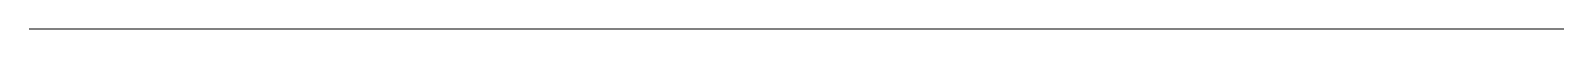
\begin{tikzpicture}
    \draw[gray,thick] (-5.5,0)--(14,0);
\end{tikzpicture}


 %%%%%%%%%%%%%%%%%%%%%%%% INICIO DEL CONTENIDO EN DOS COLUMNAS %%%%%%%%%%%%%%%%%%%%%
  
 \begin{multicols}{2\[
z(x) \, e^{\int (1-n)P(x)\,dx}
=
\int (1-n)Q(x)\, e^{\int (1-n)P(x)\,dx}\,dx + C
\]
\[
\text{y luego } y(x) = \bigl(z(x)\bigr)^{\frac{1}{1-n}}
\]
}
    \begin{center}
         \LARGE{\textbf{Capítulo I: Electrostática}}\\	
         \vspace{1.2cm}
         % \Large {Lecturers Esteban Chalbaud \& Daniel Galviz} \\
         % \large{Teaching Assistant: Mauricio Gamonal \& Irvin Martínez}\\
         % \large{PhysicsLatam.com}\\
         % \vspace{1.2cm}
         \large{25 Septiembre 2025, 6:59 am (GMT-4)}\\
         % \vspace{1.2cm}
         \large{— Ficha de Trabajo —}
    \end{center}
    %%%%%%%%%%%%%%%%%%%%%%%%%%%%excercise%%%%%%%%%%%%%%%%%%%%%%%%%%%%%%%%%%%%%%%%
    \section{luz }  
Estructuralmente, Perl está basado en un estilo de bloques como los del C o AWK, y fue ampliamente adoptado por su destreza en el procesado de texto y no tener ninguna de las limitaciones de los otros lenguajes de script. La programación es el proceso de crear un conjunto de instrucciones que una computadora puede ejecutar para realizar una tarea. Implica escribir, probar y mantener código en un lenguaje específico, como Python o JavaScript, para crear software y aplicaciones. La programación es fundamental para el desarrollo de la tecnología moderna, permitiendo la automatización de tareas y la creación de soluciones digitales
Usaremos la convención: \(r\ge 0\) (distancia radial), \(\theta\in[0,\pi]\) (ángulo polar, colatitud, medido desde el eje \(z\)) y \(\varphi\in[0,2\pi)\) (ángulo azimutal, medido en el plano \(xy\) desde el eje \(x\)).

\subsection*{Relaciones con coordenadas cartesianas}
\begin{align}
x &= r \sin\theta \cos\varphi,\\
y &= r \sin\theta \sin\varphi,\\
z &= r \cos\theta.
\end{align}

\subsection*{Relaciones inversas}
\begin{align}
r &= \sqrt{x^2 + y^2 + z^2},\\
\theta &= \arccos\!\left(\frac{z}{\sqrt{x^2+y^2+z^2}}\right)
      = \arccos\!\left(\frac{z}{r}\right),\\
\varphi &= \operatorname{atan2}(y,x).
\end{align}

\subsection*{Elementos diferenciales}
\begin{align}
\mathrm{d}\mathbf{r}\cdot\mathrm{d}\mathbf{r} &= \mathrm{d}r^{2} + r^{2}\mathrm{d}\theta^{2} + r^{2}\sin^{2}\theta\,\mathrm{d}\varphi^{2},\\
\mathrm{d}V &= r^{2}\sin\theta\,\mathrm{d}r\,\mathrm{d}\theta\,\mathrm{d}\varphi.
\end{align}

\subsection*{Vectores unitarios}
Los vectores unitarios dependientes de la posición son \(\hat{\mathbf{e}}_{r},\ \hat{\mathbf{e}}_{\theta},\ \hat{\mathbf{e}}_{\varphi}\) con orientaciones estándar radial, polar y azimutal.

\subsection*{Operadores diferenciales}
Para un campo escalar \(f(r,\theta,\varphi)\):
\begin{align}
\nabla f &= \frac{\partial f}{\partial r}\,\hat{\mathbf{e}}_{r}
          + \frac{1}{r}\frac{\partial f}{\partial \theta}\,\hat{\mathbf{e}}_{\theta}
          + \frac{1}{r\sin\theta}\frac{\partial f}{\partial \varphi}\,\hat{\mathbf{e}}_{\varphi}.
\end{align}

Para un campo vectorial \(\mathbf{A}=A_{r}\hat{\mathbf{e}}_{r}+A_{\theta}\hat{\mathbf{e}}_{\theta}+A_{\varphi}\hat{\mathbf{e}}_{\varphi}\):
\begin{align}
\nabla\cdot\mathbf{A}
&= \frac{1}{r^{2}}\frac{\partial}{\partial r}\!\left(r^{2}A_{r}\right)
 + \frac{1}{r\sin\theta}\frac{\partial}{\partial \theta}\!\left(\sin\theta\,A_{\theta}\right)
 + \frac{1}{r\sin\theta}\frac{\partial A_{\varphi}}{\partial \varphi},\\[6pt]
\nabla\times\mathbf{A}
&= \frac{1}{r\sin\theta}\left[
    \frac{\partial}{\partial \theta}\!\left(\sin\theta\,A_{\varphi}\right)
    - \frac{\partial A_{\theta}}{\partial \varphi}
  \right]\hat{\mathbf{e}}_{r}\nonumber\\
&\quad + \frac{1}{r}\left[
    \frac{1}{\sin\theta}\frac{\partial A_{r}}{\partial \varphi}
    - \frac{\partial}{\partial r}\!\left(r A_{\varphi}\right)
  \right]\hat{\mathbf{e}}_{\theta}\nonumber\\
&\quad + \frac{1}{r}\left[
    \frac{\partial}{\partial r}\!\left(r A_{\theta}\right)
    - \frac{\partial A_{r}}{\partial \theta}
  \right]\hat{\mathbf{e}}_{\varphi}.
\end{align}

La laplaciana aplicada a un escalar \(f\) queda:
\begin{align}
\nabla^{2} f
&= \frac{1}{r^{2}}\frac{\partial}{\partial r}\!\left(r^{2}\frac{\partial f}{\partial r}\right)
 + \frac{1}{r^{2}\sin\theta}\frac{\partial}{\partial \theta}\!\left(\sin\theta\frac{\partial f}{\partial \theta}\right)
 + \frac{1}{r^{2}\sin^{2}\theta}\frac{\partial^{2} f}{\partial \varphi^{2}}.
\end{align}
    \section{capitulo graciela}
Wikipedia es una enciclopedia libre,[nota 2]​ políglota y editada de manera colaborativa. Es administrada por la Fundación Wikimedia, una organización sin ánimo de lucro cuya financiación está basada en donaciones. Sus más de 63 millones de artículos en 334 idiomas han sido redactados en conjunto por voluntarios de todo el mundo,[5]​ lo que suma más de 3500 millones de ediciones, y permite que cualquier persona pueda sumarse al proyecto[6]​ para editarlos, a menos que la página se encuentre protegida contra vandalismos para evitar problemas o disputas.

Las coordenadas esféricas $(r, \theta, \varphi)$ describen la posición de un punto en el espacio mediante:

\begin{itemize}
    \item $r$: distancia del punto al origen, $r \ge 0$.
    \item $\theta$: ángulo polar, medido desde el eje $z$, $0 \le \theta \le \pi$.
    \item $\varphi$: ángulo azimutal, medido desde el eje $x$ en el plano $xy$, $0 \le \varphi < 2\pi$.
\end{itemize}

\section*{Conversión a coordenadas cartesianas}

Las relaciones entre coordenadas cartesianas $(x,y,z)$ y esféricas son:

\[
x = r \sin\theta \cos\varphi, \qquad
y = r \sin\theta \sin\varphi, \qquad
z = r \cos\theta.
\]

Las inversas son:

\[
r = \sqrt{x^2 + y^2 + z^2}, \quad
\theta = \arccos\left(\frac{z}{r}\right), \quad
\varphi = \operatorname{atan2}(y, x).
\]

\section*{Elemento de volumen}

El elemento de volumen en coordenadas esféricas se obtiene del Jacobiano:

\[
dV = r^2 \sin\theta \; dr \, d\theta \, d\varphi.
\]

\section*{Ejemplo: Volumen de una esfera}

El volumen de una esfera de radio $R$ se calcula como:

\[
V = \int_0^{2\pi}\int_0^{\pi}\int_0^R r^2 \sin\theta \; dr \, d\theta \, d\varphi
    = \frac{4}{3}\pi R^3.
\]
    \section{Capitulo Noel}    
Estructuralmente, Perl está basado en un estilo de bloques como los del C o AWK, y fue ampliamente adoptado por su destreza en el procesado de texto y no tener ninguna de las limitaciones de los otros lenguajes de script. La programación es el proceso de crear un conjunto de instrucciones que una computadora puede ejecutar para realizar una tarea. Implica escribir, probar y mantener código en un lenguaje específico, como Python o JavaScript, para crear software y aplicaciones. La programación es fundamental para el desarrollo de la tecnología moderna, permitiendo la automatización de tareas y la creación de soluciones digitales 
1. Ley de Coulomb
\section*{6. Ecuaciones de Poisson y Laplace}
Si $V$ es el potencial eléctrico:
\begin{equation}
\nabla^2 V=-\dfrac{\rho}{\varepsilon_0} \quad\text{(Ecuaci\'on de Poisson)}
\end{equation}
En regiones sin carga ($\rho=0$):
\begin{equation}
\nabla^2 V=0 \quad\text{(Ecuaci\'on de Laplace)}
\end{equation}


\section*{7. Condiciones de contorno en interfaces conductoras/diel\'ectricas}
En la superficie de un conductor en equilibrio electrost\'atico:
\begin{equation}
\mathbf{E}_{\parallel}=0, \qquad E_{\perp}=\dfrac{\sigma}{\varepsilon_0}
\end{equation}
Entre dos diel\'ectricos 1 y 2 con permitividades $\varepsilon_1,\varepsilon_2$:
\begin{align}
(\mathbf{D}_2-\mathbf{D}_1)\cdot\hat{n}&=\sigma_{f} \\
(\mathbf{E}_2-\mathbf{E}_1)\times\hat{n}&=0
\end{align}
Donde $\mathbf{D}=\varepsilon\mathbf{E}$ y $\sigma_f$ es la carga libre superficial.


\section*{8. Energ\'ia en el campo electrost\'atico}
Energ\'ia potencial de un par de cargas:
\begin{equation}
U=\dfrac{1}{4\pi\varepsilon_0}\,\dfrac{q_1 q_2}{r_{12}}
\end{equation}
Energ\'ia almacenada en un campo:
\begin{equation}
U=\dfrac{\varepsilon_0}{2}\int_{\text{all space}} E^2(\mathbf{r})\, d^3r
\end{equation}


\section*{9. Capacitancia}
Para un capacitor de placas paralelas (área $A$, separación $d$):
\begin{equation}
C=\dfrac{\varepsilon_0 A}{d}
\end{equation}
Relaci\'on general: $C=Q/V$ y energ\'ia almacenada $U=\tfrac{1}{2}CV^2$.


\section*{10. Fuerza sobre una carga en un campo eléctrico}
\begin{equation}
\mathbf{F}=q\mathbf{E}
\end{equation}


\section*{11. Distribuciones continuas comunes}
\subsection*{Línea infinita con densidad $\lambda$}
Campo a distancia radial $r$:
\begin{equation}
E(r)=\dfrac{\lambda}{2\pi\varepsilon_0 r}
\end{equation}


\subsection*{Plano infinito con densidad superficial $\sigma$}
\begin{equation}
E=\dfrac{\sigma}{2\varepsilon_0} \quad(\text{campo a cada lado del plano})
\end{equation}


\subsection*{Esfera cargada (radio $R$, carga total $Q$)}
\begin{equation}
E(r)=\begin{cases}
\dfrac{1}{4\pi\varepsilon_0}\dfrac{Q}{r^{2}} & r>R,\\[6pt]
\dfrac{1}{4\pi\varepsilon_0}\dfrac{Q r}{R^{3}} & r<R \quad(\text{si la carga est\'a distribuida uniformemente en el volumen})
\end{cases}
\end{equation}


\section*{12. Desarrollo multipolar (primeros t\'erminos)}
Potencial a gran distancia ($r\gg$ tama\~no de la fuente):
\begin{equation}
V(\mathbf{r})=\dfrac{1}{4\pi\varepsilon_0}\left(\dfrac{Q}{r}+\dfrac{\mathbf{p}\cdot\hat{r}}{r^{2}}+\dfrac{1}{2}\sum_{ij} \dfrac{Q_{ij}\hat{r}_i\hat{r}_j}{r^{3}}+\cdots\right)
\end{equation}
Donde $\mathbf{p}$ es el momento dipolar y $Q_{ij}$ el tensor cuadrupolar.


\section*{13. Imagen de cargas (ejemplo simple)}
Carga $q$ a distancia $d$ sobre un plano conductor infinito: imagen $q'=-q$ a distancia $-d$; potencial para $z>0$ equivalente al de las dos cargas.


\vspace{6pt}
\noindent\textbf{Notas finales:} Este documento contiene las ecuaciones y fórmulas principales de la electrostática clásica. Puedes usarlo como hoja de referencia para el curso o pedir que incluya ejemplos resueltos en cada sección.


    \section{capitulo max}
La Geología de Minas es la rama de la geología que se enfoca en la aplicación de principios y técnicas geológicas para el descubrimiento, exploración, evaluación, desarrollo y explotación de yacimientos de recursos minerales de manera eficiente y segura. Se apoya en disciplinas como la geotecnia y geoquímica, e integra conocimientos de geología estructural, petrología y mineralogía para entender la composición, estructura, continuidad y relaciones espaciales de las rocas que albergan los recursos, lo que es crucial para el diseño de minas y la optimización de la producción.

ECUACION DE BERNULL
\[
i\hbar \frac{\partial \Psi(\mathbf{r},t)}{\partial t}
=
\left(
-\frac{\hbar^{2}}{2m}\nabla^{2} + V(\mathbf{r},t)
\right)\Psi(\mathbf{r},t)
\]
I\[
i\hbar \frac{\partial \Psi(\mathbf{r},t)}{\partial t}
=
\left(
-\frac{\hbar^{2}}{2m}\nabla^{2} + V(\mathbf{r},t)
\right)\Psi(\mathbf{r},t)
\]
\[
i\hbar \frac{\partial \Psi(\mathbf{r},t)}{\partial t}
=
\left(
-\frac{\hbar^{2}}{2m}\nabla^{2} + V(\mathbf{r},t)
\right)\Psi(\mathbf{r},t)
\]
 
\[
p + \tfrac{1}{2}\rho v^{2} + \rho g h = \text{constante}
\]
\[
p_1 + \tfrac{1}{2}\rho v_1^{2} + \rho g h_1
=
p_2 + \tfrac{1}{2}\rho v_2^{2} + \rho g h_2 + \rho g h_f
\]
\[
z(x) \, e^{\int (1-n)P(x)\,dx}
=
\int (1-n)Q(x)\, e^{\int (1-n)P(x)\,dx}\,dx + C
\]
\[
\text{y luego } y(x) = \bigl(z(x)\bigr)^{\frac{1}{1-n}}
\]
\[
z(x) \, e^{\int (1-n)P(x)\,dx}
=
\int (1-n)Q(x)\, e^{\int (1-n)P(x)\,dx}\,dx + C
\]
\[
\text{y luego } y(x) = \bigl(z(x)\bigr)^{\frac{1}{1-n}}
\]
\[
i\hbar \frac{\partial \Psi(\mathbf{r},t)}{\partial t}
=
\left(
-\frac{\hbar^{2}}{2m}\nabla^{2} + V(\mathbf{r},t)
\right)\Psi(\mathbf{r},t)
\]
\[
i\hbar \frac{\partial \Psi(\mathbf{r},t)}{\partial t}
=
\left(
-\frac{\hbar^{2}}{2m}\nabla^{2} + V(\mathbf{r},t)
\right)\Psi(\mathbf{r},t)
\]

    \section{Capitulo rulo}
Perl es un lenguaje de programación diseñado por Larry Wall en 1987. Perl toma características del lenguaje C, del lenguaje interpretado bourne shell, AWK, sed, Lisp y, en un grado inferior, de muchos otros lenguajes de programación.
Sea \( f(x) = x^2 + 2x + 1 \). Entonces:

\[
f(x) = (x+1)^2
\]

La derivada es:

\[
f'(x) = 2x + 2
\]
    \section{Capitulo Anais}
Strawberry Perl is a perl environment for MS Windows containing all you need to run and develop perl applications. It is designed to be as close as possible to perl environment on UNIX systems.
    
    \input{sections/std/hugo.tex}
   


\end{multicols}
